\documentclass[11pt,a4paper]{article}

\usepackage[T1]{fontenc}
\usepackage[utf8]{inputenc}
\usepackage[english]{babel}
\usepackage[sc]{mathpazo}
\linespread{1.05}
\usepackage{microtype}
\usepackage[a4paper,margin=2.5cm]{geometry}
\usepackage{amsmath,amssymb}
\usepackage{graphicx}
\usepackage{booktabs,tabularx}
\usepackage{enumitem}
\usepackage[font=small,labelfont=bf,labelsep=colon]{caption}
\usepackage{xcolor}
\usepackage[most]{tcolorbox}
\usepackage[hidelinks]{hyperref}

\definecolor{blueI}{HTML}{2A78D6}
\newtcolorbox{summary}{enhanced, breakable, colback=blueI!5!white, colframe=blueI, boxrule=0pt,
  leftrule=2.4pt, arc=0pt, outer arc=0pt, left=6pt, right=6pt, top=3pt, bottom=3pt}

\title{\textbf{Tuning the group identification}\\[4pt]
  \large How the delay $\delta$, the false discovery rate $q$ and the duration $\tau^*$\\
  were chosen on the FFVL archive}
\author{Matteo Di Sante}
\date{Working note, 21 October 2026\\[2pt]
  \small Companion of the note \emph{Group flights in free flight} (same folder)}

\begin{document}
\maketitle

\begin{summary}
\textbf{The choice.} Two pilots are in contact when one of them passes within
$\varepsilon_h=500$~m and $\varepsilon_z=300$~m of where the other was at most
$\delta=2$~min before or after; headings are compared only when both glide
($\theta_{\max}=45^\circ$) and gaps shorter than $g=120$~s are joined. A contact counts
when it lasts at least $\tau^*=38.1$~min, the shortest duration at which chance explains at
most $q=0.1$ of the contacts kept. With these values 21.7\% of the paraglider flights and
6.9\% of the hang-glider flights fly in a group at some point, in 17\,169 episodes.

\textbf{Why.} The delay was measured: real pairs have 3.7 to 5.7 times the correspondences
of chance within 2~min, less beyond (Section~\ref{sec:delta}). $\tau^*$ is not set by
hand: it follows from $q$ and from the null model (Section~\ref{sec:fdr}); $q$ is the
trade-off between how many groups we see and how many of them are chance
(Section~\ref{sec:q}).

\textbf{Where.} \nolinkurl{/Volumes/SSD_DISANTE/xc-lab/group-identification/runs/d120_eh500_ez300_th45_g120_q0.1},
with a \texttt{PARAMETERS.md} that lists every parameter.
\end{summary}

\tableofcontents

\section{What is tuned}

The method of the companion note has three kinds of parameters
(Table~\ref{tab:parameters}). The \emph{tolerances} say when two positions match:
$\delta$, $\varepsilon_h$, $\varepsilon_z$, $\theta_{\max}$, $g$. The \emph{duration}
$\tau^*$ says how long a match must last to be a contact; it is not chosen directly but
computed from the share $q$ of chance contacts we accept. The other \emph{settings} make the
computation exact or fast and are fixed by physical bounds.

\begin{table}[h]
\centering
\small
\begin{tabularx}{\textwidth}{@{}l l X@{}}
\toprule
Parameter & Value & How it was set \\
\midrule
$\delta$, largest delay & 2 min & measured: delay profile, Section~\ref{sec:delta} \\
$q$, accepted false discovery rate & 0.1 & trade-off, Section~\ref{sec:q} \\
$\tau^*$, shortest contact & 38.1 min & computed from $q$ and the null model, Section~\ref{sec:fdr} \\
$\varepsilon_h$, $\varepsilon_z$ & 500 m, 300 m & definition of ``the same air'' (companion note); sensitivity in Section~\ref{sec:sensitivity} \\
$\theta_{\max}$ & 45$^\circ$ & no effect on the result (Section~\ref{sec:sensitivity}) \\
$g$, longest gap joined & 120 s & starting value of the note; sensitivity in Section~\ref{sec:sensitivity} \\
$\Delta$, $h_{\max}$, $R_\mathrm{dep}$, $v_{\max}$, $R_s$, $r_{\min}$ & see Section~\ref{sec:fixed} & physical bounds and exactness \\
\bottomrule
\end{tabularx}
\caption{The parameters and how each was set.}
\label{tab:parameters}
\end{table}

\section{Chance contacts and $\tau^*$}\label{sec:fdr}

Two pilots who never interact still meet: they take off from the same site, follow the same
ridges and valleys and climb in the same house thermals. The null model of the companion
note measures how often. For pairs of flights of the same day whose takeoffs are less than
$R_s=10$~km apart, one flight is replaced by its copy shifted in time by more than $2\delta$,
so that every real correspondence is destroyed while routes and thermals stay the same. The
contacts of these surrogate pairs are chance. On date $d$, with $\rho_{0,d}(\tau)$ the
surrogate intervals lasting at least $\tau$ per second of surrogate exposure and $H_d$ the
exposure of the real pairs (the time both flights fly after departure), chance gives
$\sum_d \rho_{0,d}(\tau) H_d$ intervals lasting at least $\tau$. With $N(\tau)$ the real ones,
\begin{equation}\label{eq:fdr}
  \widehat{\mathrm{FDR}}(\tau)=\frac{\sum_d \rho_{0,d}(\tau)\,H_d}{N(\tau)},\qquad
  \tau^*=\min\bigl\{\tau:\ \widehat{\mathrm{FDR}}(\tau)\le q\bigr\}.
\end{equation}

\begin{figure}[h]
\centering
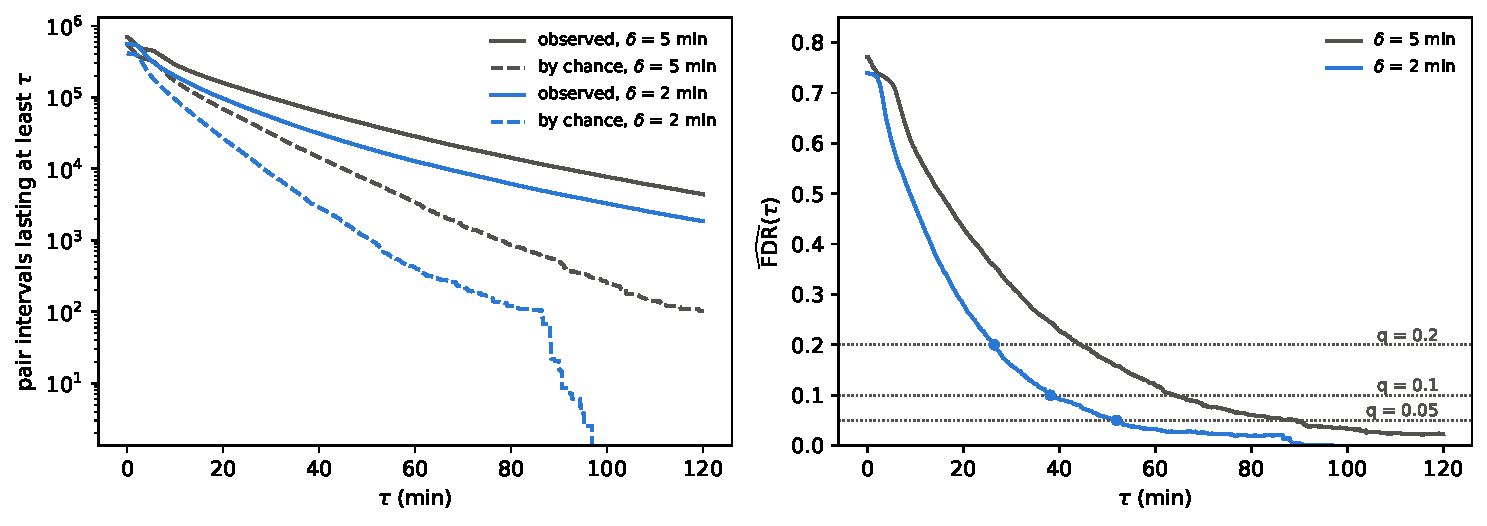
\includegraphics[width=\textwidth]{figures/tuning_fdr.pdf}
\caption{Left: real pair intervals lasting at least $\tau$ (solid) and those chance alone
gives (dashed), with $\delta=5$~min (grey) and $\delta=2$~min (blue), on the whole archive.
Right: their ratio, the false discovery rate of Eq.~\eqref{eq:fdr}; dots mark $\tau^*$ for
$q=0.05$, 0.1 and 0.2 with $\delta=2$~min.}
\label{fig:fdr}
\end{figure}

Figure~\ref{fig:fdr} is the central fact of the tuning. Most contacts are chance: 74\% of all
pair intervals with $\delta=2$~min (77\% with 5~min), 47\% of those lasting 10~min, 16\% of
those lasting 30~min. Short contacts therefore say little; only long ones are mostly real.
This is why $\tau^*$ is tens of minutes: it is the duration at which the real contacts
outnumber chance by the factor $1/q$. Resampling the dates 200 times moves $\tau^*$ by a
few minutes (Table~\ref{tab:q}), so the curve, not the noise of the surrogates, sets it.

\section{The delay $\delta$}\label{sec:delta}

\subsection{The delay profile}

A wider $\delta$ catches pilots who follow farther behind, but it also adds chance
correspondences. To see where the signal ends, we counted, for every delay $l$, the
correspondences $(t,t+l)$ of the real pairs and of the surrogate pairs, per second of
exposure, with a window of 15~min on 300 random dates (58\,910~h of real exposure):
\begin{equation}\label{eq:profile}
  R(l)=\frac{\text{real correspondences at delay } l \text{ per second of exposure}}
             {\text{chance correspondences at delay } l \text{ per second of exposure}} .
\end{equation}

\begin{figure}[h]
\centering
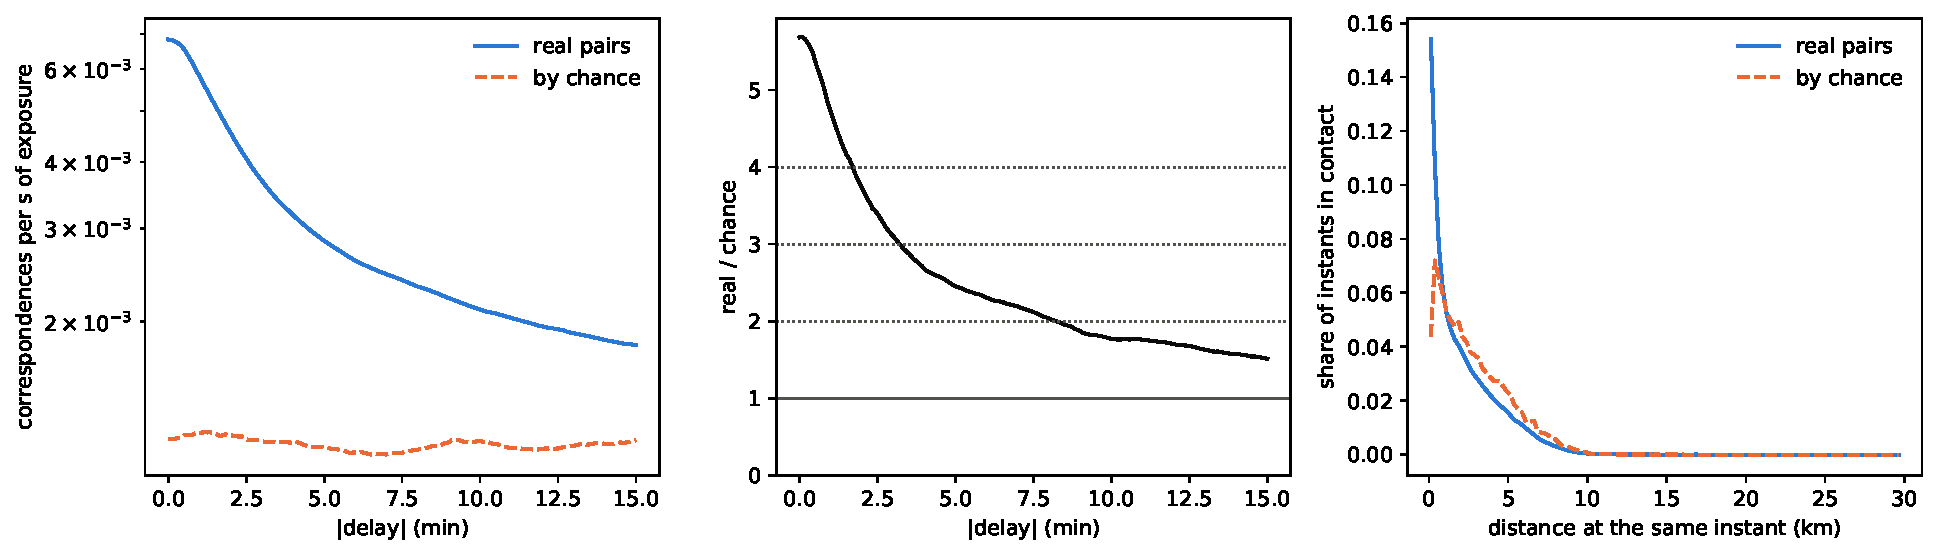
\includegraphics[width=\textwidth]{figures/tuning_delays.pdf}
\caption{The delay profile on 300 dates with a 15~min window. Left: correspondences per
second of exposure at each delay, real and by chance. Middle: their ratio $R(l)$ of
Eq.~\eqref{eq:profile}, with the levels 4, 3 and 2. Right: the distance between the two
pilots at the same instant when one is on the path of the other.}
\label{fig:delays}
\end{figure}

Chance is flat in the delay, as it should: a shifted copy has no preferred delay. The real
pairs peak at a few seconds, where they have 5.6 times the correspondences of chance, and
decay: $R$ falls below 4 at 105~s, below 3 at 195~s and below 2 at 500~s, and is still 1.5 at
15~min (Figure~\ref{fig:delays}). The excess has two parts. The fast one, within 2--3~min, is
pilots flying together. The slow one, which has not ended at 15~min, is pilots who use the
same thermals at about the same time of day without following each other: the shift of the
null model, more than 30~min with this window, removes that synchronisation too. A rule such
as ``the delay that holds 95\% of the excess'' would pick 13~min, because it counts the slow
tail; that is why we read the ratio instead.

\subsection{The delay inside the long contacts}

The contacts that survive $\tau^*$ tell the same. Figure~\ref{fig:ell} shows, for the pair
intervals of the run with $\delta=5$~min, the median delay between the two pilots inside each
interval. Short intervals pile up at the edge of the window, 300~s: 29\% of those under
10~min, the signature of chance matches, which are spread over all delays and are found at
the largest ones. Long intervals do not: those of at least 90~min have a median delay of
25~s, 90\% of them within 2~min, and only 6 of 10\,734 at the edge.

\begin{figure}[h]
\centering
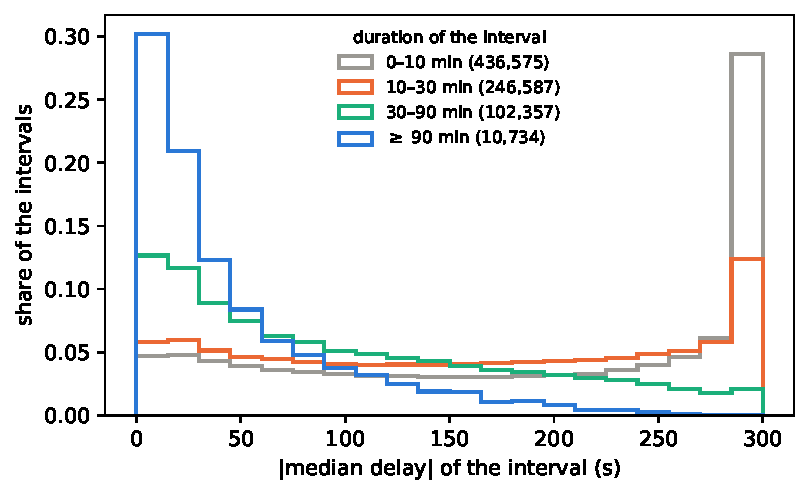
\includegraphics[width=0.62\textwidth]{figures/tuning_ell.pdf}
\caption{Median delay between the two pilots inside each pair interval, by the duration of
the interval ($\delta=5$~min, whole archive).}
\label{fig:ell}
\end{figure}

\subsection{The choice}

We take $\delta=2$~min: within it the real correspondences are at least 3.7 times chance, and
it contains nine in ten of the long contacts. Shortening the delay also shortens $\tau^*$, since
fewer chance matches enter: from 89.5 to 51.9~min at $q=0.05$ (Table~\ref{tab:q}).

The delay also bounds how far apart two pilots in contact can be at the same instant: at most
$\varepsilon_h+v_{\max}\delta\approx0.5+27.8\times120/1000\approx3.8$~km. A
separation of 6~km, the largest we want to call a group, is never reached by one pair; a
group, a chain of pairs, can be wider. Even with the 15~min window, 58\% of the instants in
contact have the two pilots within 2~km and 94\% within 6~km (Figure~\ref{fig:delays},
right).

\section{The false discovery rate $q$}\label{sec:q}

$q$ is the share of chance contacts we accept among those we keep. A smaller $q$ keeps only
very long contacts and few groups, all of them real; a larger $q$ sees more groups, with more
chance among them. Table~\ref{tab:q} and Figure~\ref{fig:q} give the trade-off.

\begin{table}[h]
\centering
\small
\begin{tabular}{@{}l l c c c c c@{}}
\toprule
$\delta$ & $q$ & $\tau^*$ (min) & 5--95\% over dates & para in a group & hang in a group & episodes \\
\midrule
5 min & 0.05 & 89.5 & 79.5--91.5 & 8.9\% & 2.1\% & 6\,090 \\
2 min & 0.05 & 51.9 & 49.1--53.3 & 13.7\% & 3.8\% & 10\,553 \\
2 min & 0.1  & 38.1 & 37.0--41.1 & 21.7\% & 6.9\% & 17\,169 \\
2 min & 0.2  & 26.4 & 25.2--27.2 & 31.7\% & 13.9\% & 26\,504 \\
\bottomrule
\end{tabular}
\caption{$\tau^*$ and the groups it gives. Flights with a logger of at most 10~s and a
position after departure: 154\,598 paragliders and 6\,039 hang gliders.}
\label{tab:q}
\end{table}

\begin{figure}[h]
\centering
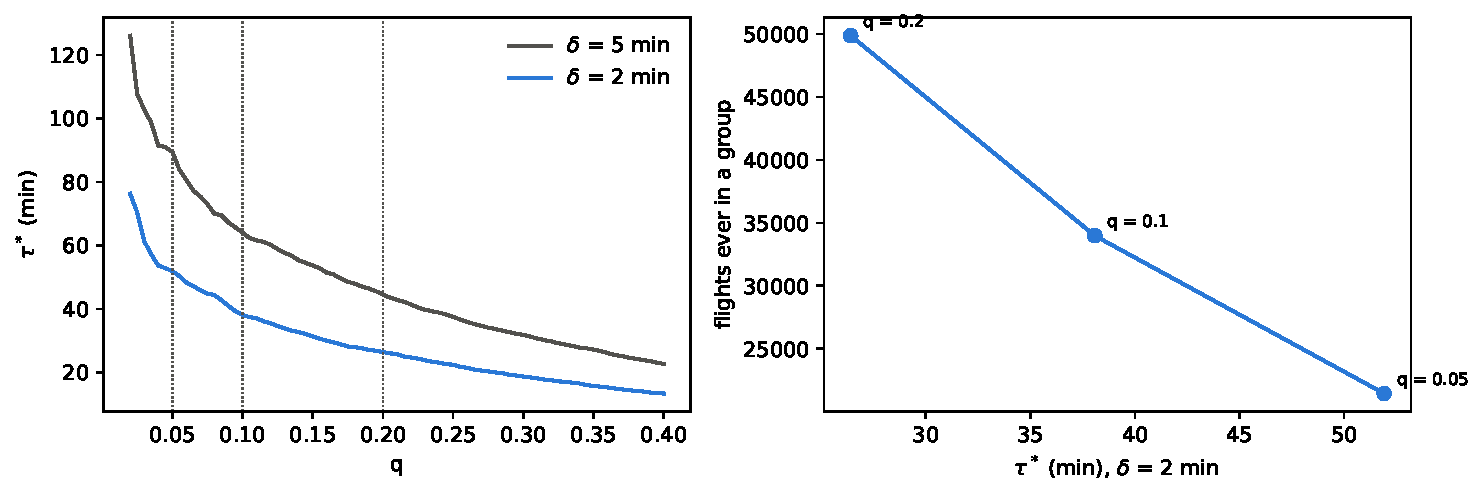
\includegraphics[width=\textwidth]{figures/tuning_q.pdf}
\caption{Left: $\tau^*$ as a function of $q$, for the two delays. Right: flights ever in a
group against $\tau^*$, for $q=0.05$, 0.1 and 0.2 with $\delta=2$~min.}
\label{fig:q}
\end{figure}

We take $q=0.1$: at most one contact in ten is chance, and $\tau^*=38.1$~min. Going to 0.2 would
lower $\tau^*$ to 26~min but would let chance make one group in five.

\section{Sensitivity to the other tolerances}\label{sec:sensitivity}

The companion note asks for a plateau: values of the tolerances around which the result does
not change. We changed one parameter at a time on 300 random dates, recalibrating $\tau^*$
each time, with $\delta=5$~min (Table~\ref{tab:plateau}). $\theta_{\max}$ changes nothing:
contacts in glide are few. The others move the fraction of flight time in a group, $f_G$, by
up to a factor three, mostly through $\tau^*$: there is no plateau, so the tolerances are
definitions to declare rather than values the data single out. On 300 dates $\tau^*$ is
noisy (126~min with the starting values against 89.5 on the whole archive, and six settings
stop at the same surrogate interval); a conclusive check needs the whole archive for each
setting, about one hour each. It was not repeated with $\delta=2$~min.

\begin{table}[h]
\centering
\small
\begin{tabular}{@{}l c c c c@{}}
\toprule
Setting ($\delta=5$ min unless stated) & $\tau^*$ (min) & $f_G$ & episodes & flights in a group \\
\midrule
starting values & 126.1 & 0.034 & 98 & 210 \\
$\varepsilon_h=250$ m & 75.1 & 0.058 & 253 & 537 \\
$\varepsilon_h=1000$ m & 126.8 & 0.065 & 162 & 372 \\
$\varepsilon_z=150$ m & 126.1 & 0.020 & 61 & 125 \\
$\varepsilon_z=600$ m & 126.1 & 0.044 & 122 & 268 \\
$\delta=2$ min & 42.6 & 0.106 & 600 & 1\,170 \\
$\delta=10$ min & 128.4 & 0.062 & 153 & 365 \\
$\theta_{\max}=30^\circ$ & 126.1 & 0.034 & 97 & 208 \\
$\theta_{\max}=90^\circ$ & 126.1 & 0.034 & 98 & 210 \\
$g=60$ s & 75.8 & 0.087 & 332 & 732 \\
$g=300$ s & 126.1 & 0.055 & 141 & 318 \\
\bottomrule
\end{tabular}
\caption{One parameter at a time on 300 random dates (7\,051 flights), $q=0.05$.}
\label{tab:plateau}
\end{table}

\section{Fixed settings}\label{sec:fixed}

\begin{itemize}[leftmargin=1.2em]
\item $\Delta=5$~s, the common grid: a pilot is at most 69~m from a grid position at
  100~km/h, against $\varepsilon_h=500$~m.
\item $h_{\max}=10$~s: positions are interpolated only between fixes at most 10~s apart; the
  flights of coarser loggers are left out of the statistics.
\item $R_\mathrm{dep}=3$~km: contacts around the takeoff, before the first exit from this disc,
  are not counted.
\item $v_{\max}=100$~km/h, the speed of the candidate filter: pieces of track end at every
  faster step, so the filter never misses a correspondence (checked against every pair of
  instants on synthetic days).
\item $R_s=10$~km, $r_{\min}=2\delta+\Delta$, at most 200 surrogate pairs per date: the null
  model of Section~\ref{sec:fdr}.
\end{itemize}

\section{Limits}

\begin{itemize}[leftmargin=1.2em]
\item The null model shifts tracks by more than $2\delta$, which also removes the
  synchronisation of pilots with the weather of the day. What it calls real therefore includes
  pilots who share the same thermal at the same time without following each other: the
  ``same air'' notion of the companion note, not proof of interaction.
\item $\varepsilon_h$ and $\varepsilon_z$ are definitions; a distance profile, the analogue of
  Figure~\ref{fig:delays} for the horizontal and vertical gap, would measure them as the delay
  was measured.
\item The plateau of Section~\ref{sec:sensitivity} is on 300 dates and with the old delay.
\item The data are the cleaned tracks of the old repository (soaring, tag
  \texttt{legacy-final}); the phases needed by the heading condition exist on 1~Hz flights
  only.
\end{itemize}

\end{document}
